\documentclass[class=article, crop=false]{standalone}
\usepackage[subpreambles=true]{standalone}
\usepackage{import}
\usepackage{preamble}
\usepackage{pdfpages}
\begin{document}
\begin{figure}[h]
    \caption{Cross-correlations of indicators, coloured by industry group}
    \hspace{-18pt}
    \begin{subfigure}{\textwidth}
        \centering
        \vspace{-100pt}
        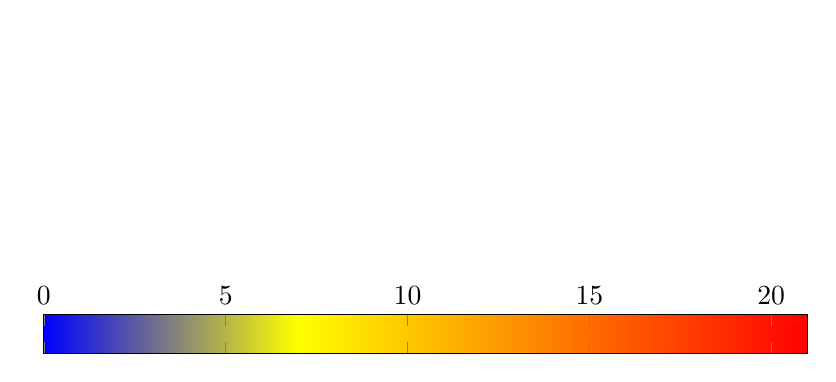
\begin{tikzpicture}
        \begin{axis}[
        hide axis,
        scale only axis,
        colorbar horizontal,
        point meta min=0,
        point meta max=21,
        colorbar style={
            width=0.8\textwidth,
            xtick={0,5,...,21},
            ylabel style={},
            xticklabel pos=upper,
            at={(0.0,0.0)},anchor=north west
            }
         ]
        \addplot[draw=none] coordinates {(0,0)};
        \end{axis}
        \end{tikzpicture}
    \end{subfigure}
    %Male ----------------------------------
    \begin{subfigure}{0.3\textwidth}
        \import{graphs/}{m_wpremium-percnonwhite}
        \caption{Male}
        \label{fig:m_wpremium-percnonwhite}
    \end{subfigure}
    \hspace{-10pt}
    \begin{subfigure}{0.3\textwidth}
        \import{graphs/}{m_wpremium-percracist}
        \caption{Male}
        \label{fig:m_wpremium-percracist}
    \end{subfigure}
    \hspace{-10pt}
    \begin{subfigure}{0.3\textwidth}
    \centering
        \import{graphs/}{m_percnonwhite-percracist}
        \caption{Male}
        \label{fig:m_percnonwhite-percracist}
    \end{subfigure}
    % \hfill
    % \begin{subfigure}{0.1\textwidth}
    %     \hfill
    % \end{subfigure} 
    %Female ----------------------------------
    \begin{subfigure}{0.3\textwidth}
        \import{graphs/}{f_wpremium-percnonwhite}
        \caption{Female}
        \label{fig:f_wpremium-percnonwhite}
    \end{subfigure}
    \begin{subfigure}{0.3\textwidth}
        \import{graphs/}{f_wpremium-percracist}
        \caption{Female}
        \label{fig:f_wpremium-percracist}
    \end{subfigure}
    \begin{subfigure}{0.3\textwidth}
    \centering
        \import{graphs/}{f_percnonwhite-percracist}
        \caption{Female}
        \label{fig:racist_nonwhite}
    \end{subfigure}
    %\begin{subfigure}{0.1\textwidth}
     %   \hfill
    %\end{subfigure} 
    \vspace{-30pt}
    \label{fig:cross_correls}
\end{figure}
\end{document}